%=======================================================================
\chapter[Multi-paradigm programming in Prolog and .NET]{Multi-paradigm program-\\ming in Prolog and .NET}
\label{ch:mpp-in-dotnet}
%=======================================================================

\tuprolog{}.NET now provides the user with the same features as the Java version, extending and specializing the multi-paradigm, multi-language experience to the plethora of languages available onto the Microsoft .NET platform.
In this Chapter, the impact of such change is discussed, both in terms of specific conceptual concepts (namely, \textit{language conventions} to handle multiple languages) and new/specialized libraries and predicates to be used for language interaction.

Since the current status of \tuprolog{}.NET depends \textit{a)} on its past history and \textit{b)} on the IKVM tool \cite{ikvm}, the two following Sections summarize its evolution from version 2.1 and the basics of IKVM translation, respectively.

While their reading is recommended to everyone, the reader wishing only to exploit \tuprolog{}.NET in its current version can safely bypass them and jump directly to Section \ref{sec:dotnet-tuprolog-now}.

%-----------------------------------------------------------------------
\section{A bit of history}
\label{sec:dotnet-tuprolog-history}
%-----------------------------------------------------------------------

%--------------------------------------------
\subsection{\tuprolog{} 2.1 and CSharpLibrary}
\label{ssec:dotnet-tuprolog2.1}
%--------------------------------------------

\tuprolog{}.NET appeared as a usable tool for the first time in April 2007, with the .NET conversion of \tuprolog{} 2.1; an earlier, experimental version had been made with version 2.0, but was never officially published.

tuProlog.NET 2.1 run on Microsoft .NET 2.0 and on Mono 1.2.5\footnote{The MONO version required a source tuning for the \texttt{TheoryManager.find} method.}, and was a complete rewriting in C\# of the original Java code: the executable became a .NET \texttt{exe} file, and all the libraries became .NET \texttt{dll} assemblies.

The Java-based, key feature to multi-paradigm-programming, \textit{JavaLibrary}, was replaced by a corresponding \textit{CSharpLibrary}, which provided the very same features, except for a few syntactic changes:
\begin{itemize}
  \item any \texttt{java\_\textit{xxx}} predicate was renamed as \texttt{csharp\_\textit{xxx}}.

  \item C\# objects defined in other namespaces than \texttt{System} required that the new namespace be explicitly passed to the predicate creating the object: so, \texttt{java\_object/3} became \texttt{csharp\_object/4}:\\
        \texttt{csharp\_object(\textit{\textbf{AssemblyName}}, \textit{ClassName}, \textit{ArgumentList}, \textit{ObjRef})}\\
      Moreover, the assembly containing the definition of the object type must be in the same folder as the \texttt{alice-tuProlog.dll} file.

\item an \textit{ad hoc} predicate was added for array creation, instead of using the standard \texttt{csharp\_object/3}-\texttt{/4} resulting from the direct conversion of JavaLibrary predicates:
    \texttt{csharp\_array(\textit{AssemblyName}, \textit{Type}, \textit{Length}, \textit{ObjRef})}
\end{itemize}

An annoying limitation concerned the loading of user-defined libraries (and theories), which had to be in the same folder as the \tuprolog{} (\texttt{IDE.exe} or \texttt{CUIConsole.exe}) executable.

From the developers' viewpoint, using \tuprolog{} classes in a Visual Studio project required a reference to the \texttt{alice-tuProlog.dll} assembly be added to the project, and the \texttt{tuProlog} namespace be imported in the usual C\# fashion (e.g. \texttt{using tuProlog;}).

%--------------------------------------------
\subsection{\tuprolog{} 2.1.3: CSharpLibrary + exceptions}
\label{ssec:dotnet-tuprolog2.1.3}
%--------------------------------------------

As a further step towards the convergence of the .NET and Java versions, the ``\tuprolog{} 3'' project --later renamed as 2.1.3 -- was started to add the exceptions support, being developed for the Java version, to the .NET version, too.
However, this version was never officially released, because of the quasi-simultaneous
development of \tuprolog{} 2.2, whose \textit{CLILibrary} could provide a much larger interest from the multi-paradigm, multi-language viewpoint.

%--------------------------------------------
\subsection{\tuprolog{} 2.2 and CLILibrary}
\label{ssec:dotnet-tuprolog2.2}
%--------------------------------------------

Version 2.2\footnote{%
    Unfortunately, version numbering for .NET was incoherent with the Java version at that time: in Java, 2.2 was the version that introduced the exception support, which was absent in 2.2 for .NET because the development \tuprolog{} 2.1.3, where exceptions were being added, occurred quasi-simultaneously, but not in time for the two projects to converge. In addition, this version was never tested on Mono.
} was a milestone in \tuprolog{}.NET history, as it generalized \textit{CSharpLibrary} to enable multi-language programming with \textit{virtually any language available on the .NET platform}, rather than C\# only (unfortunately, it lacked exception support, due to the race between the two quasi-simultaneous projects).

To this end, the concept of \textit{Language Convention} was introduced to encapsulate the language-specific aspects, so that a single library -- renamed \textit{CLILibrary} instead of \textit{CSharpLibrary} -- could handle any language.
%
Each convention contains the syntax conversion operations and the post-compilation transformations required for a given language.
Conventions were developed for C\#, J\#, VisualBasic.NET, F\#, Eiffel.NET and
IronPythonStudio.

Following the generalization renaming of \textit{CSharpLibrary} as \textit{CLILibrary}, a few syntactic changes were also made:
\begin{itemize}
  \item any \texttt{csharp\_\textit{xxx}} predicate of CSharpLibrary was renamed here as \texttt{cli\_\textit{xxx}}; this applies both to predicates derived from the JavaLibrary (of the form \texttt{java\_\textit{xxx}}) and to predicates added by CSharpLibrary, like \texttt{csharp\_array/4};

 \item to create objects bound to a particular \textit{Convention}, the \texttt{cli\_object/5} predicate was introduced whose first argument specifies the convention to be used:\\
     \texttt{cli\_object(\textit{\textbf{Convention}}, \textit{AssemblyName}, \textit{ClassName},\\
     \mbox{~~~~~~~~~~~}\textit{ArgumentList}, \textit{ObjRef})}

 \item furthermore, for those .NET programming languages whose constructor function is not constrained to coincide with the class name, and therefore require such a name to be explicitly specified on object creation, the \texttt{cli\_object/6} predicate was introduced:\\
     \texttt{cli\_object(\textit{Convention}, \textit{AssemblyName}, \textit{ClassName},\\
     \mbox{~~~~~~~~~~~}\textbf{\textit{ContructorName}}, \textit{ArgumentList}, \textit{ObjRef})}

 \item two convention handling predicates, also usable as directives, were introduces to load/unload conventions to/from a Prolog theory:\\
     \texttt{load\_convention(\textit{Assembly}, \textit{ConventionName}, \textit{ConventionAtom})}\\
     \texttt{unload\_convention(\textit{ConventionAtom})}.
\end{itemize}

From the developers' viewpoint, the new aspect is how to define new conventions: this is done by starting a new project (class library), importing the \texttt{alice-tuprolog.dll} reference and implement a new class extending \texttt{tuProlog.Convention} in the \texttt{tuProlog.Conventions} namespace.

The \texttt{dll} generated by the compilation must then be moved to the main project compiling folder.


%--------------------------------------------
\section{IKVM Basics}
\label{sec:dotnet-ikvm}
%--------------------------------------------

IKVM.NET \cite{ikvm} is basically a .NET implementation of Java (language, infrastructure, tools) enriched with special tools for Java/.NET conversion.
Its distribution, which adheres to the \textit{zlib} open source license, includes:
\begin{itemize}
  \item a .NET implementation of a Java Virtual Machine;
  \item a Java class library, based on OpenJDK, re-implemented in .NET;
  \item tools for Java/.NET inter-operability---in particular, the \texttt{ikvmc} bytecode translator that converts Java bytecode to Microsoft .NET Common Intermediate Language (CIL).
\end{itemize}

\noindent Both Microsoft .NET 2.0 and Mono platforms 2.0 are supported, both for \textit{x86} and \textit{x64} architectures. If necessary, the source pack is also available.

Debugging is also very well supported: if the Java sources are available, proper information can be generated\footnote{The option must be specified to generate the \texttt{pdb} (\textit{Program Debug Database}) file, to be copied to the application folder in Visual Studio.} that enable Microsoft Visual Studio to keep the .NET and and Java sources in sync, following the program execution on the Java source, too, as well as enabling breakpoints, variable inspection, etc.

%--------------------------------------
\subsection{Dynamic vs. Static modality}
\label{ssec:ikvm-dynamic-static}
%--------------------------------------

IKVM can work in two modalities. In the \textit{dynamic} modality, Java applications are converted in .NET on-the-fly and immediately executed; in the \textit{static} modality, instead, Java applications (or libraries) are translated into a .NET assembly, to be used to develop a .NET native application.

The dynamic modality is supported by the \texttt{ikvm} tool, which is analogous to Java's \texttt{java} interpreter\footnote{Most command line options work identically with both tools.}: so, a Java application can be executed in .NET as in would be in a Java-enabled machine, just replacing \texttt{java} with \texttt{ikvm}, in a totally user-transparent way.

The class loading mechanisms in this modality behaves exactly as in Java, with the class path options.
The only drawback is performance, which is obviously penalized by the on-the-fly translation.

The static modality is supported by the \texttt{ikvmc} tool, which generates a \texttt{dll} or \texttt{exe} .NET assembly (depending whether the translation concerns a Java library or application, respectively) converting Java types to .NET types.
Obviously, this tool has no Java counterpart: its options control the target architecture (\textit{x86} or \textit{x64}), the kind of output (\texttt{dll}/\texttt{exe}), etc.
Unlike the previous case, here the Java class loading mechanisms has some limitations, that are discussed below.
One possible drawback is IKVM choice of translating the Java \textit{package} visibility into .NET \textit{internal}'s, making it impossible to access such properties and methods from other assemblies (even though they were accessible in the Java architecture).

%--------------------------------------
\subsection{Class loading issues}
\label{ssec:ikvm-class-loading}
%--------------------------------------

The class loading mechanism is perhaps the major issue when translating Java applications to .NET, because of the very different approach adopted by the two architectures, which makes it difficult to define a general mapping. In fact,
\begin{itemize}
  \item the Java approach is based on the \textit{class path} concept, which defines the set of paths where classes must be looked for;
  \item the .NET approach, instead, exploits the current folder, the Global Assembly Cache (GAC) and configuration files for the same purpose.
\end{itemize}

\noindent In order to bridge this gap, IKVM adopts the following intelligent approach:
\begin{itemize}
  \item each \textit{statically-generated} assembly is associated to its own class loader---either a user-supplied one, or the default one;

  \item the default class loader looks for classes:
  \begin{enumerate}
    \item first, in the assembly itself;
    \item then, in all the assemblies \textit{directly referenced} by the former.
  \end{enumerate}
\end{itemize}

\noindent This approach guarantees that classes are always found \textit{if all dependencies are statically expressed}, i.e. if all the libraries used by an application are statically known, and their references are added in the application project.
Problems are to be expected, instead, for dynamically loaded classes, whose references were not included in the project---and whose assemblies, therefore, are not considered by the class loader.

To overcome this issue, four alternatives can be followed:
\begin{enumerate}
  \item creating a \textit{single assembly}, if size is not a problem and run-time modularity is irrelevant (that is, loading all modules even when just one is actually used is irrelevant);
  \item adding a static reference (\texttt{-r} option) to the library to be dynamically loaded, when the application is translated to .NET: then, the default .NET loading will locate the library, but the need to specify all its details (including version number) cancels most of the advantage of dynamic loading, since any change in the library to be loaded still requires a rebuild;
  \item using the special \texttt{ikvm.runtime.AppDomainAssemblyClassLoader}
  class loader provided by IKVM;
  \item writing an ad-hoc class loader, typically extending \texttt{URLClassLoader}: this is perhaps the most flexible, but also the user-heaviest, solution.
\end{enumerate}

\noindent One further interesting aspect is that the IKVM implementation of Java's \texttt{Class.forName} method adopts a more general behavior than Java's default implementation, supporting the dynamic loading of classes also \textit{beyond} the current assembly even without special options, provided that their \texttt{AssemblyQualifiedName} is specified; otherwise, only the current assembly is checked.

So, a Java application that exploited \texttt{Class.forName} for dynamic class loading, that could originally load only classes in the application JAR unless properly launched (see Section \ref{ssec:library-loading-issues}), will be able to load .NET\footnote{The reason why this feature is limited to .NET classes is, trivially, that only .NET classes possess the \texttt{AssemblyQualifiedName} property and the other assembly details (version, culture, public key token).} classes beyond the application's own assembly when translated to .NET via IKVM.

For the above reason, the \texttt{set\_classpath/1} and \texttt{get\_classpath/1} predicates available in \tuprolog{} for Java are \textit{not} available for .NET classes, as they refer to the class loading mechanism available in Java only, which remains ``behind the scenes'' in \tuprolog{}.NET only for Java parts translated to .NET via IKVM.

%--------------------------------------
\subsection{The other way: writing .NET applications in Java}
\label{ssec:ikvm-writing-app-in-java}
%--------------------------------------

Beyond converting Java applications in .NET, IKVM also supports the opposite direction---that is, writing .NET applications \textit{in Java}, as if this were one of .NET-supported languages.

This feature is provided by the \texttt{ikvmstub} tool, which generates a Java JAR archive from a .NET assembly (\texttt{dll}/\texttt{exe}).
As the tool name suggests, the generated JAR is just a stub, containing all the Java classes and interfaces corresponding to the .NET originals, but no actual implementation, since this will be written directly in Java: its purpose is just to satisfy the \texttt{javac} compiler's type checking, and enable the code completion feature on the IDE (e.g. Eclipse) used for the Java application development.

In this way, a Java application can be written (in Java---using Eclipse, Netbeans, etc.)) that exploits the .NET types extracted from the .NET original assemblies.
This application can be compiled with \texttt{javac} as usual, specifying the above stub JAR in the class path (\texttt{-cp} option).

Obviously, such an application can \textit{not} be run in Java with the standard \texttt{java} interpreter, as the above stub JAR does not contain any actual implementation---nor would that be reasonable, since the goal was to exploit Java to write a .NET application, not a Java one.
%
Instead, the resulting ``fake'' Java application is to be translated via \texttt{ikvmc}, and then executed \textit{in .NET} where the original assemblies provide the ``missing'' classes.

\medskip

In this context, .NET concepts are mapped onto suitable Java concepts by \texttt{ikvmstub} as follows:
\begin{itemize}
  \item \textit{namespaces} are mapped onto Java packages, pre-pending the \texttt{cli.} prefix to prevent name clashes;
  \item \textit{properties} are mapped onto a pair of Java \texttt{\textit{get}}/\texttt{\textit{set}} methods;
  \item \textit{enumerations} are mapped onto classes extending \texttt{cli.System.Enum}, with static fields with integer values for each possible value of the .NET enumerative type;
      % MAYBE IN THE FUTURE THIS WILL CHANGE, AND ENUM WILL BE USED.
  \item \textit{delegates} are mapped onto a Java class and a nested helper \texttt{Method} interface: the class derives from \texttt{System.MulticasDelegate} and has the same name as the original delegate, while the nested interface always declares an \texttt{Invoke} method whose signature matches the delegate: this method is called when an event occurs. This is why, the class constructor takes as its argument an object implementing the \texttt{Method} interface, whose implementation of \texttt{Invoke} does the actual job.
  \item \textit{events} are mapped onto a pair of Java \texttt{\textit{add\_*}}/\texttt{\textit{remove\_*}} methods, whose argument is an object of the class representing the delegate;
  \item \textit{params} is mapped onto an array of \texttt{Object}s;
          % MAYBE IN THE FUTURE THIS WILL CHANGE, AND GENERICS WILL BE USED.
  \item \textit{attributes} are mapped onto a Java class with the same name as the .NET attribute, plus a pair of Java \texttt{\textit{get}}/\texttt{\textit{set}} methods for each property defined by the attribute.\footnote{The java class also includes a nested Java annotation, called \texttt{Annotation}, which defines Java methods homonomous to the .NET attribute properties: any reference to such an annotation in the Java code will be translated into the corresponding .NET attribute when the application is converted to .NET. However, only read properties are supported, even if the original .NET attribute properties were read/write.}
\end{itemize}

%-----------------------------------------------------------------------
\section{\tuprolog.NET now}
\label{sec:dotnet-tuprolog-now}
%-----------------------------------------------------------------------

The management difficulties in keeping coherent two such evolving projects (the Java and the .NET versions) indicated that the approach of a separate development was not sustainable in the perspective.
This led to a complete strategic change, resulted into the adoption of the IKVM \cite{ikvm} bytecode translator as a tool to automate the generation of \tuprolog.NET \textit{from the same Java bytecode} (other than sources) as the Java version, which could then become the only one to be actively maintained ``by hand''.

Despite some (minor) performance issues (the IKVM-generated \tuprolog{} version appears 15\% slower, in the average, than its Java counterpart), the approach turned out to be winning, enabling the two platforms to converge for all they have in common---namely, everything other than the \textit{CLILibrary} and the .NET-specific issues.

%--------------------------------------------
\subsection{Highlights}
\label{ssec:dotnet-highligths}
%--------------------------------------------

From version 2.5, \tuprolog{}.NET builds on top of the winning idea of version 2.2 (language conventions for multi-language interoperability with Prolog), but goes farther by exploiting the value-added brought by the IKVM approach: the chance to use \textit{even Java} as if it were directly available on the .NET platform.
%
This extra value spreads into several directions:
\begin{itemize}
  \item .NET objects can be accessed, in addition to Java objects, via .NET-specific \textit{OOLibrary} -- a specialisation of the Java version of OOLibrary -- from \tuprolog{};

  \item .NET applications can be developed (instead of Java applications, which obviously require the \tuprolog{} Java version) that exploit \tuprolog{} as a third-party library, with the only difference that a \texttt{dll} assembly is to be referenced by the (Visual Studio) project, instead of a JAR archive;

  \item the whole P@J framework for implementing Java methods in Prolog remains available, and takes a newer form in the .NET context;

  \item \tuprolog{} libraries can be written in Java, as well as in other .NET languages, resulting into a \texttt{dll} assembly in the end;

  \item Java can be used together with C\#, F\#, and other .NET languages in the same .NET application, where \tuprolog{} can possibly play the role of the director (orchestrator, coordinator) in-front-of or behind the scenes.
\end{itemize}

\noindent In the next Sections of this Chapter, these dimensions are discussed and explored, roughly following the same structure as Chapter \ref{ch:mpp-in-java}.

\begin{table}
{\small
\begin{tabular}{|p{2cm}|p{2cm}|p{2.4cm}|p{2cm}|p{2.2cm}|}
\hline
  Benchmark & Java direct & Java via Prolog & C\# direct & C\# via Prolog\\
  Math   & 118 & 182 & 116 & 118\\
  Concat & 185 & 211 & 162 & 161\\
  Sort   & 147 & 149 & 142 & 143\\
  \hline
\end{tabular}}
  \caption{Performance comparison between Java and C\# code executed directly or via \tuprolog{}.NET (times in milliseconds).}\label{tab:dotnet-benchmarks}
\end{table}

From the performance viewpoint, the experience of the older \tuprolog{}.NET 2.2 (see Section \ref{ssec:dotnet-tuprolog2.2}) showed that an overhead is to be expected on Java applications.
To quantify it in some common situations, Table \ref{tab:dotnet-benchmarks} shows the average execution times of three micro-benchmarks (\textit{math}, \textit{concat} and \textit{sort}) when written in Java and C\#, executed directly and via \tuprolog{}.NET, respectively: \textit{math} performs algebraic operations on real numbers, \textit{concat} concatenates strings via the \texttt{StringBuilder} class available in both languages, and \textit{sort} sorts an array of integer numbers via quicksort.

Quite clearly, the execution of Java code via IKVM introduces an overhead\footnote{These figures are not very sensitive to the time overhead of class loading, because the classes to be loaded here are few and small: however, the first iterations of the test program do show higher execution times for this reason.} whose weight depends of the specific operation area, and whose cause is mainly the IKVM implementation of Java libraries: in fact, the \textit{sort} test, where IKVM incorporates its own implementation of the Java library instead of using the default one, is not affected in its performance.

Conversely, the execution of .NET code (the implementation language selected is irrelevant for this comparison) is basically overhead-free even when triggered from \tuprolog{}.

%-----------------------------------------------------------------------
\section{Using .NET from Prolog: OOLibrary}
\label{sec:dotnet-oolibrary}
%-----------------------------------------------------------------------

\subsection{Motivation}

Since \tuprolog{}.NET is automatically generated from the Java sources via IKVM, the ``Java based'' OOLibrary (formerly known as JavaLibrary) is also available for free; however, since this library was designed for Java, it inherently supports Java concepts and constructs, but is obviously unaware of the features that are specific to .NET languages, such as properties, delegates, etc.
%
So, while .NET objects could be loaded and exploited via OOLibrary ``as is'' (thanks to the extended semantics of \texttt{Class.forName} discussed in Section \ref{ssec:ikvm-class-loading}), their support would be imperfect, for three main reasons:
\begin{itemize}
  \item the lack of support for some .NET language constructs;
  \item the different Java naming convention for methods w.r.t. Java;
  \item the code reorganisation performed behind-the-scenes by the .NET compilers, which sometimes change the names of syntactic elements---for instance, properties are compiled by adding a pair of getter/setter methods.
\end{itemize}

\noindent These aspects are put well in evidence by the example below, which refers to a class \texttt{Student} (written in C\#) defining a ``standard'' student with some ``obvious'' properties:

\begin{verbatim}
    new_object('CStudent.Student, CStudent',
                [123456,'John','Smith'], Obj),
    Obj <- 'PrintStudent' returns Value,
    Obj <- 'get_Name' returns Value,
    Obj <- 'set_Name'('Albert').
\end{verbatim}

\noindent As the first line shows, a \texttt{Student} instance can be created via \texttt{new\_object/3} \textit{as if it were a Java class}, but only by means of its \texttt{\textit{AssemblyQualifiedName}}---possibly specifying also its version, culture and public key.
Moreover, the method name must be quoted, since the .NET conventions require the first letter to be capitalized.
Last but not least, access to properties -- that the translated OOLibrary does not know  as such -- must be mediated by the get/set methods added by the .NET compiler, with a loss both of expressiveness (the \texttt{Obj.Property} notation is lost) and of transparency (the compiler transformations must be known to bypass the problem).

This is why \tuprolog{}.NET defines its own \textit{OOLibrary}, which specialises the ``Java'' one and is therefore loaded by default in place of its Java counterpart. 
As shown in Figure \ref{fig:dotnet-oolibrary}, to be compared with Figure \ref{fig:gui-library-manager} on page \pageref{fig:gui-library-manager}, the Library Manager dialog here lists the .NET version of OOLibrary, instead of the Java version, as its first item.

\begin{figure}
\centering
  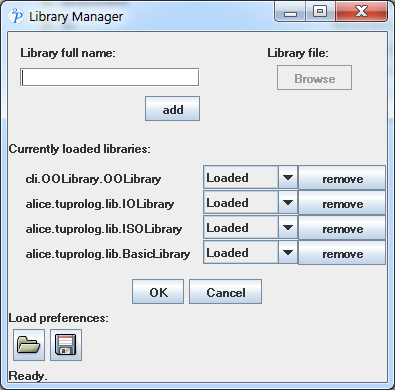
\includegraphics[width=8cm]{images/dotnet-oolibrary}
  \caption{Library manager in tuProlog.NET: notice the .NET library version of OOLibrary loaded.}\label{fig:dotnet-oolibrary}
\end{figure}

The .NET version of OOLibrary extends the underlying Java version by enabling \tuprolog{}.NET to interact with both Java and .NET software components. In principle, any .NET language can be supported, although the current distribution includes the support only for the most widely used .NET languages (C\#, F\# and VB.NET), other than Java itself; however, the support for other .NET languages can be easily added, by defining further \textit{language conventions}.

\subsection{Language Conventions}

Language conventions are \tuprolog{} means to separate and embed the language-specific aspects from the library core: originally introduced in \tuprolog{}.NET 2.2 (see Section \ref{ssec:dotnet-tuprolog2.2} above), they work as a bridge between the language-specific naming issues and the underlying Java-based machinery.

Conventions define standard methods (Table \ref{tab:dotnet-convention-interface}) that express how the name of the required entity (class, method, property, public field, etc) must be modified to take into account the compiler modifications, so that the original .NET name may be transparently used in a \tuprolog{} program.
%
\begin{table}
{\small
\begin{verbatim}
public abstract class Convention{
  public abstract string Name ...
  public virtual string GetNamespace(string oldNamespace) ...
  public virtual string GetClassName(string oldClassName) ...
  public virtual string GetMemberName(string oldMemberName) ...
  public virtual string GetFieldName(string oldFieldName) ...
  public virtual string GetPropertyGetterName(string oldPropName) ...
  public virtual string GetPropertySetterName(string oldPropName) ...
  public virtual bool IsArrayClass(string className)...
  public static Convention LoadConvention(string assembly,
                                          string className)...
}
\end{verbatim}
}
\caption{The public interface of the root \texttt{Convention} class. Any actual convention for a given language must specialize from this class according to the language details.}
\label{tab:dotnet-convention-interface}
\end{table}
%
Obviously, the \texttt{GetXX} methods convert the name of the corresponding entity, while \texttt{IsArrayClass} checks whether the class represents an array---typically verifying if its name ends with \texttt{"[]"}, but this behavior can be redefined if a language adopts a different naming scheme.
The abstract \texttt{Name} property represents the name of the convention: each actual convention will set it to the corresponding language (i.e., \texttt{"csharp"}, \texttt{"fsharp"}, etc.)

Currently, four conventions are included in the distribution:
\begin{itemize}
  \item \textbf{C\#}: in this language all the names, except for field names, must start with a capital letter: so the \texttt{GetXX} methods must change the letter case accordingly. Moreover, since properties are compiled in a pair of \texttt{get\_}/\texttt{set\_} methods, the two \texttt{GetPropertyGetterMethod} and \texttt{GetPropertySetterMethod} methods return strings like \texttt{get\_\textit{PropName}} / \texttt{set\_\textit{PropName}}, respectively.

  \item \textbf{F\#}: this convention is identical to C\#'s.

  \item \textbf{VB.NET}: this convention is identical to C\#'s, except for arrays, that are defined through \texttt{()} in Visual Basic .NET instead of \texttt{[]}: so, the \texttt{IsArrayClass} method is redefined accordingly.

  \item \textbf{Java} this convention operates opposite to the above, changing method and field names so that they start with a lowercase letter; class names are checked for starting with an uppercase letter, and packages are changed to all-lowercase.
\end{itemize}

\noindent Since conventions and OOLibrary are part of \tuprolog{}.NET only, they are both implemented in C\#, to avoid unnecessary intermediate conversions.

\subsection{.NET-specific OOLibrary Predicates}

OOLibrary puts together the easy of use and immediateness of the Java version of OOLibrary with the convention-based inspiration of the former \textit{CLILibrary} (found in version 2.2): Table \ref{tab:dotnet-oolibrary-interface} lists its predicates.
%
\begin{table}
{\small
\begin{verbatim}
public class OOLibrary {
  public bool new_object_3(Term className,
                           Term args, Term objRef)
  public bool new_object_4(Term conventionName, Term className,
                           Term args, Term objRef)
  public bool new_object_4(Term conventionName, Term className,
                           Term constructorName, Term args, Term objRef)
  public bool destroy_object_1(Term objRef)
  public bool method_call_3(Term objRef, Term methodName, Term resRef)
  public bool load_convention_3(Term assemblyName,
                                Term conventionName, Term convRef)
  public bool dload_convention_3(Term assemblyName,
                                Term conventionName, Term convRef)
  public bool unload_convention_1(Term convRef)
}
\end{verbatim}
}\caption{The public interface of the \texttt{OOLibrary} class. In addition, the \texttt{$<-$/2}, (\texttt{$<-$},\texttt{returns})\texttt{/3} and \texttt{.} operators are defined for method calling and field/property access with the \texttt{get}/\texttt{set} pseudo-methods, exactly as in Java's OOLibrary.}
\label{tab:dotnet-oolibrary-interface}
\end{table}

\noindent These methods modify the names of the received entities according to the specified convention, then call the corresponding methods of the underlying Java's OOLibrary.
For instance, if the target object is written in C\#, OOLibrary:
\begin{itemize}
  \item retrieves the associated convention (if any);
  \item changes the method name accordingly;
  \item invokes \texttt{java\_call\_3} to perform the operation.
\end{itemize}

\noindent The \texttt{dload\_convention\_3} method is the directive version of \texttt{load\_convention\_3}), the difference being in the lifetime of the loaded convention: the directive loads a convention for the whole life of the current \tuprolog{} engine, while the standard version loads it for the duration of the current query only.

%-------------------------------------
\subsubsection{Convention Examples}
\label{sec:dotnet-oolibrary-examples}
%-------------------------------------

%To show OOLibrary at work, it is first necessary to start \tuprolog{}.NET and \textit{manually remove JavaLibrary} (loaded by default as a side effect of the translation from Java) via the Library Manager, and then and \textit{manually add OOLibrary} by typing the string \texttt{OOLibrary.OOLibrary, OOLibrary} in the Library Manager's textfield, and pressing the \textit{Add} button. A confirmation message should appear, confirming that OOLibrary is now loaded.

The \texttt{Student} class (already cited in Section \ref{sec:dotnet-oolibrary}) has been rewritten in all the four supported languages:
Tables \ref{tab:dotnet-oolibrary-examples1} shows how it can be exploited from \tuprolog{}.NET in Visual Basic (top two examples) and Java (bottom two examples), with and without conventions, while Table \ref{tab:dotnet-oolibrary-examples2} shows a comprehensive example where all the four supported .NET languages are used at the same time by the same \tuprolog{} program.

\begin{table}
{\small
\begin{verbatim}
visualbasicWithoutConvention :-
  new_object('VBStudent.Student',[123456, john, smith], Obj),
  Obj <- 'PrintStudent' returns Student,
  Obj <- get_Id returns StudentNumber,
  class('VBStudent.Student,VBStudent') <- get_StaticProperty returns Value,
  new_object('VBStudent.Student, VBStudent[]',[10], Array).

visualbasicWithConvention :-
  load_convention('VBConvention.dll','VBConvention.VBDotNet',Conv),
  new_object(Conv,'VBStudent.Student, VBStudent',
                                     [123456, john, smith], Obj),
  Obj <- printStudent returns Student,
  Obj.id <- get(StudentNumber),
  class('VBStudent.Student, VBStudent').staticProperty <- get(Value),
  new_object(Conv, 'VBStudent.Student, VBStudent()',[10], Array).

javaWithoutConvention :-
  new_object('javastudent.Student',[123456, john, smith], Obj),
  Obj <- printStudent returns Student,
  Obj <- getId returns StudentNumber,
  class('javastudent.Student') <- printInfoUniv returns University,
  new_object('javastudent.Student[]',[10], Array).

javaWithConvention :-
  load_convention('JavaConvention.dll','JavaConvention.Java',Conv),
  new_object('javastudent.Student',[123456, john, smith], Obj),
  Obj <- 'PrintStudent' returns Student,
  Obj <- getId returns StudentNumbers,
  class('javastudent.Student') <- printInfoUniv returns University,
  new_object('javastudent.Student[]',[10], Array).
\end{verbatim}
}
  \caption{Using the \texttt{Student} class in Visual Basic and Java without / with conventions.}
  \label{tab:dotnet-oolibrary-examples1}
\end{table}

\noindent Without conventions (Table \ref{tab:dotnet-oolibrary-examples1}), syntax is heavier and less natural from the viewpoint of the language considered.
In the first example, for instance, \textit{i)} method names must be quoted because of their capital initial, \textit{ii)} accessing a property means to know the corresponding method name (\texttt{get\_Id}), and \textit{iii)} array creation calls for an ``absurd'' (from the VB.NET viewpoint) \texttt{[]} suffix instead of the \texttt{()} used in that language for that purpose.
Using the VB convention, instead, method quoting is no longer necessary, property access can be made in a straightforward way (\texttt{Object.Property} notation), and array .creation adheres to the Visual Basic syntax rules.


Similar considerations apply to Java objects, too: in this case, either the Java class is translated in .NET statically (in which case the corresponding \texttt{dll} will be available in the file system), or the Java \texttt{.class} file is kept ``as is'', and is loaded and converted dynamically by IKVM when needed\footnote{via the \texttt{ClassPathAssemblyClassLoader} (Section \ref{ssec:ikvm-class-loading}).}
In this case the convention is perhaps less necessary, since the naming changes imposed by the language style are minimal; yet, the convention makes it possible to write method names with the lowercase initial, making the Prolog writing lighter.

Table \ref{tab:dotnet-oolibrary-examples2}) shows two examples of such situations, whose run is shown in Figure \ref{fig:dotnet-tokenizer-and-dynamic-compilation}: the top one instantiates a \texttt{StringTokenizer} object, using IKVM's implementation of that class (whose \texttt{dll}, therefore, is statically available), and uses it to scan a string, while the bottom one is a case of dynamic compilation of a Java source: the source is compiled by IKVM on the fly into a \texttt{dll}, which is then loaded and used as appropriate---here, to open a file chooser dialog and return the selected file name (see the output tab in the GUI).

\begin{table}
{\footnotesize
\begin{verbatim}
useJavaClassAsIs :-
  new_object('java.util.StringTokenizer', ['This is my string'], Tokenizer),
  Tokenizer <- nextToken returns Token1,
  write(Token1), nl.

dynamicCompilation :-	
  java_class('public class MyClass {
     public String showFileChooser(String title) {
      javax.swing.JFileChooser chooser = new javax.swing.JFileChooser();
      chooser.setDialogTitle(title);
      chooser.showOpenDialog(null);
      java.io.File file = chooser.getSelectedFile();
      return file.getName();
     }
    }',
   'MyClass', [], C),
  new_object('java.lang.String',['Select a file from tuProlog!'], Message),
  C <- newInstance returns Object,
  Object <- showFileChooser(Message) returns FileName,
  write(FileName).
\end{verbatim}
}
  \caption{Using the Java \texttt{StringTokenizer} straight from \tuprolog{}.NET \textit{(top)} and dynamically compile a Java source, convert it to \texttt{dll}, and use it directly to instantiate an object and exploit it \textit{(bottom)}. See also Figure \ref{fig:dotnet-tokenizer-and-dynamic-compilation}.}
  \label{tab:dotnet-oolibrary-examples2}
\end{table}

\begin{figure}
  \centering
  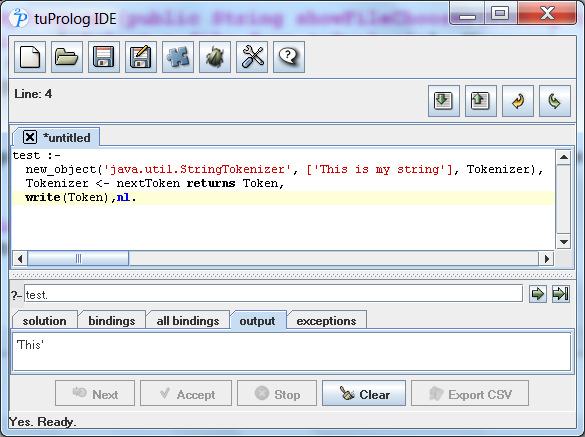
\includegraphics[width=11cm]{images/dotnet-oolibrary-using-StringTokenizer.png}
  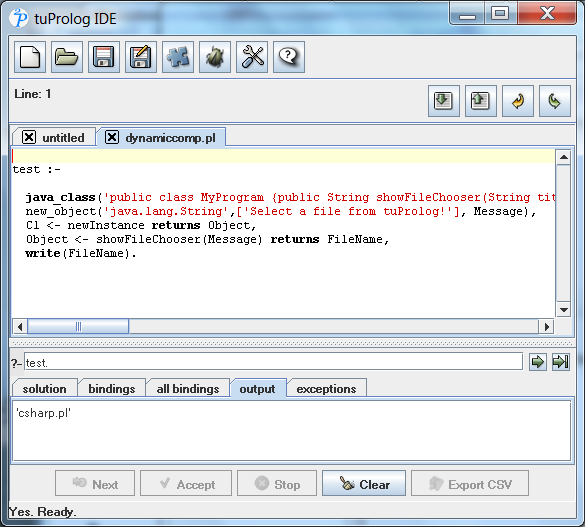
\includegraphics[width=11cm]{images/dotnet-oolibrary-dynamiccompilation.png}
  \caption{\tuprolog{}.NET executing the example in Table \ref{tab:dotnet-oolibrary-examples2}. Of course, the execution time of the second example is sensible, since \texttt{ikvm} is triggered behind the scenes to compile the class source.}\label{fig:dotnet-tokenizer-and-dynamic-compilation}
\end{figure}


Table \ref{tab:dotnet-oolibrary-examples3}) shows one further example, where \tuprolog{} instantiates and exploits objects written in multiple languages, \textit{maintaining the interoperability between Prolog primitive types (string, numbers, etc) and the primitive types of the .NET and Java languages}.
In fact, values in the Prolog variables \texttt{Ex1}, \texttt{Ex2}, \texttt{Ex3} and \texttt{Ex4} are summed directly, with no explicit conversions.

\begin{table}
{\footnotesize
\begin{verbatim}
sumAllExams(TotExams) :-
 load_convention('CSharpConvention.dll','CSharpConvention.CSharp',CSConv),
 load_convention('FSharpConvention.dll','FSharpConvention.FSharp',FSConv),
 load_convention('VBConvention.dll',    'VBConvention.VBDotNet',  VBConv),
 load_convention('JavaConvention.dll',  'JavaConvention.Java',    JConv),

 new_object(CSConv, 'CStudent.Student, CStudent',[122345,'john',''], StudCS),
 new_object(FSConv, 'FStudent.Student, FStudent',[525718,'Mary',''], StudFs),
 new_object(VBConv, 'VBStudent.Student, VBStudent',[987650,'Jean',''], StudVB),
 new_object(JConv,  'javastudent.Student',[476328,'Holly',''], StudJa),

 StudCS.exams <- get(Ex1),
 StudFs.exams <- get(Ex2),
 StudVB.exams <- get(Ex3),
 StudJa <- getExams returns Ex4,

 TotExams is Ex1 + Ex2 + Ex3 + Ex4.
\end{verbatim}
}
  \caption{Using four \texttt{Student} classes written in four languages.}
  \label{tab:dotnet-oolibrary-examples3}
\end{table}

Interoperability between .NET and Java classes becomes a problem, instead, when complex types (i.e., anything other than primitive types) are involved in the same \tuprolog{} program, because a Java object, possibly returned from a Java method, cannot be passed to a .NET instance ``as is'', and no automatic conversion occurs.
%
The typical workaround to this problem is to transform the problematic data in suitable Prolog strings that constitute a valid \tuprolog{} representation of a value of a Prolog type (and viceversa), thus exploiting \tuprolog{} as a mediator (both as a component and as a language) to overcome the incommunicability.
%
This issue is covered more in detail in Section \ref{sec:dotnet-putting-together} below.

%-------------------------------------
\subsection{Lambda expressions in .NET}
\label{ssec:dotnet-oolibrary-lambdas}
%-------------------------------------

Perhaps surprisingly, the complex machinery behind the lambda expression handling in the Java-based OOLibrary is perfectly translated by IKVM, and works seamlessly in such a different host environment as Microsoft .NET.

However, the precise semantics of the lambda operator \texttt{'<-'} in such a multi-language environment -- which includes both any .NET language \textit{and Java} -- needs to be pointed out.
From this viewpoint, it must be kept in mind that, since \tuprolog{}.NET derives from the Java version via IKVM translation,  \textit{the lambda operator \texttt{'<-'} maintains the Java 8 semantics even in this environment}--- which means, among the other things, to live with Java 8 functional interfaces as target types.

Of course, we are well aware that this is might sound a little awkward to .NET programmers, who are used to lambda constructs based delegates as target types: hopefully, a .NET-specific lambda treatment will be added some time in the future.

%-------------------------------------
\subsection{Handling .NET Exceptions}
\label{ssec:dotnet-oolibrary-exceptions}
%-------------------------------------

Since the .NET OOLibrary is rooted on the underlying Java's OOLibrary, exceptions raised during the execution of methods on .NET objects accessed from Prolog behave exactly as in the Java case (see Section \ref{ssec:java-exceptions-in-tuprolog})---that is, \textit{.NET exceptions are never perceived as such: rather, they are encapsulated in some Java exception.}

Accordingly, these exceptions are handled in \tuprolog{}.NET via the same \texttt{java\_catch/3} predicate defined in Section \ref{ssec:java-exceptions-in-tuprolog} for the Java version: syntax and use are identical to the Java case, too.

For instance, let us suppose that the \texttt{Counter} class has been defined in .NET, and we wish to intercept the case that the class is not available at run time for loading. This means that the OOLibrary's \texttt{new\_object} predicate could fail to load the class, raising an exception.
In a standard .NET environment, the exception raised would be a .NET \texttt{TypeNotFoundException}, but \textit{this is not the case here, because the mediation of IKVM encapsulates such events and re-throws them as Java exceptions.}
As a result, a \texttt{java.lang.ClassNotFoundException} has to be matched against, as in the following example:

\begin{verbatim}
test:-
  java_catch( new_object('Counter',[], c),
    [ ('java.lang.ClassNotFoundException'(Cause, Msg, _),
        write(Msg) )],
    write('+++') ).
\end{verbatim}
%
This is why the predicate name remains \texttt{java\_catch}, as in the Java version of OOLibrary -- in fact, it captures Java exceptions only.

Figure \ref{fig:dotnet-exceptions} shows the above examples and the corresponding output in the \tuprolog{} GUI.
%
\begin{figure}
\centering
  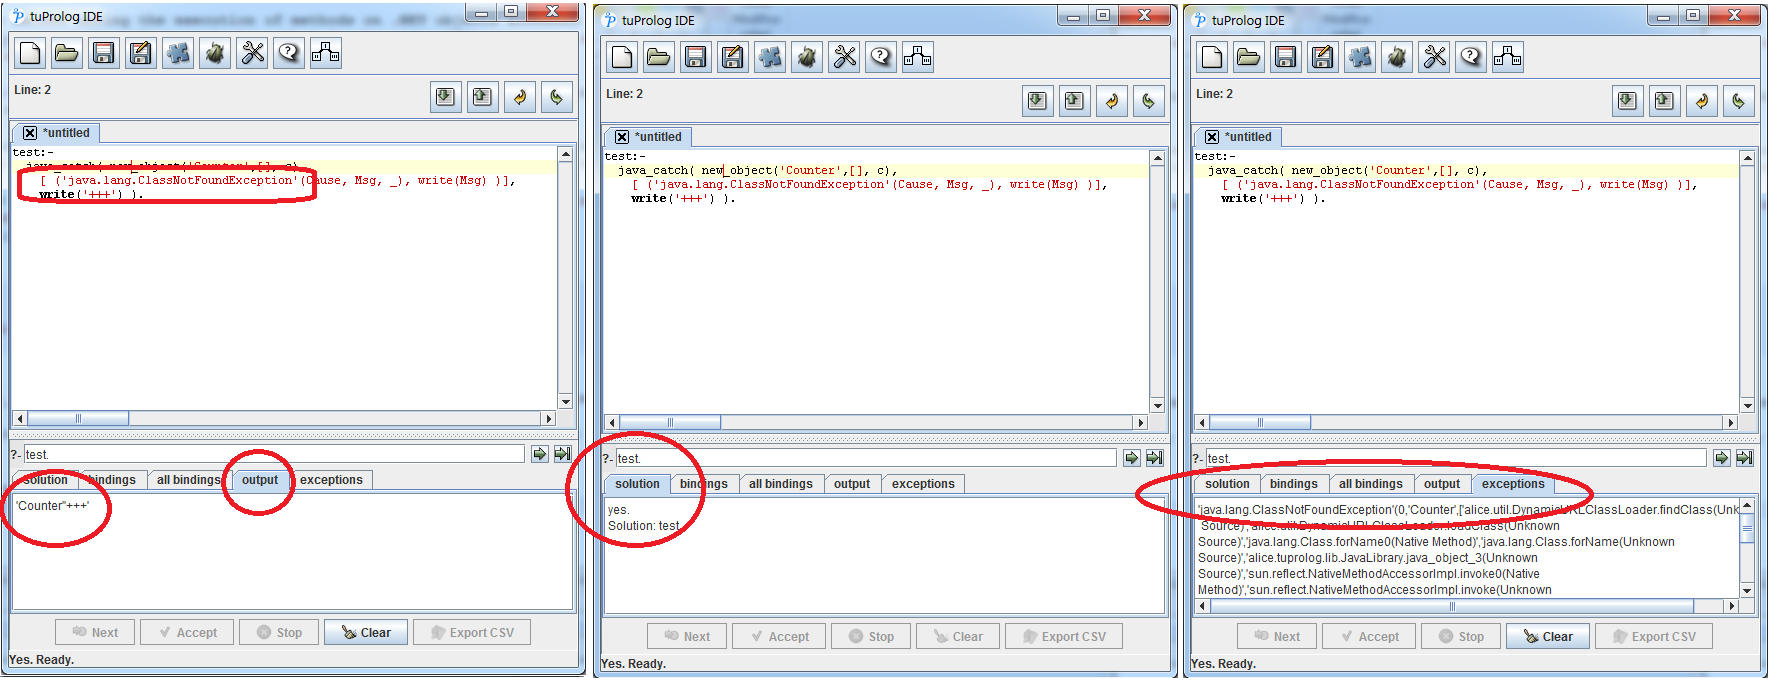
\includegraphics[width=12cm]{images/dotnet-exceptions}
  \caption{\texttt{java\_catch} example in .NET}\label{fig:dotnet-exceptions}
\end{figure}
%
However, please note that this is by no way a definitive choice, since future developments might include the ability to trap .NET exceptions natively.

For further examples, the interested reader can refer to Section \ref{ssec:java-exception-examples} on page \pageref{ssec:java-exception-examples}, where Java-related exceptions are presented and discussed.



%-----------------------------------------------------------------------
\section{Using Prolog from .NET: the API}
\label{sec:dotnet-oo-api}
%-----------------------------------------------------------------------

Since \tuprolog{}.NET is automatically generated from the Java sources via IKVM, the available API is the same presented in Section \ref{sec:java-api}.
%
To create a .NET application using \tuprolog{}, do the following:\footnote{The example is taken from the degree thesis in Computer Engineering of Alessandro Montanari, Universit\`{a} di Bologna, 2010.}

\begin{enumerate}
  \item open the IDE of your choice (we refer to Microsoft Visual Studio 2010);
  \item create a new project (in our case, from the \textit{File} menu, select \textit{New $>$ Project}), select the proper language (in this case, \textit{Visual C\#} from the left panel), the proper application type (here, \textit{Windows Forms Application}), and digit the application name and file position (Figure \ref{fig:dotnet-visualstudio1}, \textit{top});
  \item add a reference to the \tuprolog{}.NET assembly, \texttt{tuprolog.dll} (in this case, right-click on \textit{References} in the \textit{Solution Explorer} panel, click on \textit{Add References}, browse the file system up to the assembly and select it---Figure \ref{fig:dotnet-visualstudio1}, \textit{bottom});
  \item add a reference to the \texttt{IKVM.OpenJdk.Core.dll} assembly that contains the IKVM implementation of Java packages, following the same procedure;
  \item now write/draw your .NET application (in this case, we draw the user interface shown in Figure \ref{fig:dotnet-visualstudio3} (\textit{top}) and write the implementation of the \textit{OK} button \ref{fig:dotnet-visualstudio4}); the final result (an application for the symbolic derivative of a function, where Prolog takes care of the symbolic calculus and .NET of the GUI) is shown in Figure \ref{fig:dotnet-visualstudio3} (\textit{bottom}).
\end{enumerate}

\begin{figure}
\centering
  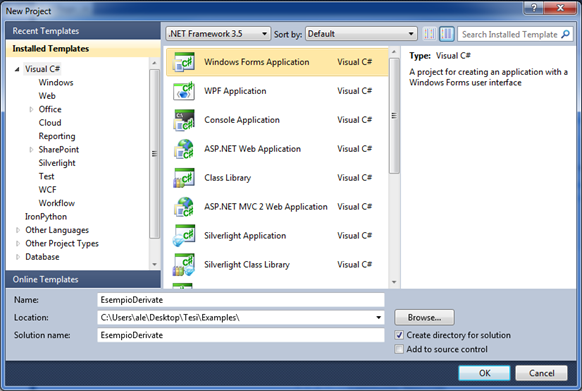
\includegraphics[width=12cm]{images/dotnet-visualstudio1}\\
  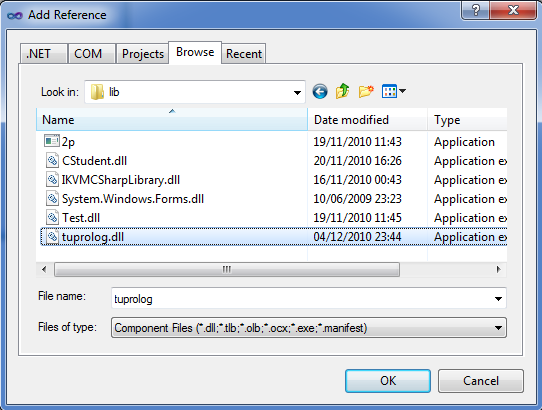
\includegraphics[width=12cm]{images/dotnet-visualstudio2}
  \caption{Creating a .NET application using \tuprolog{} in Visual Studio: new project.}\label{fig:dotnet-visualstudio1}
\end{figure}

\begin{figure}
\centering
  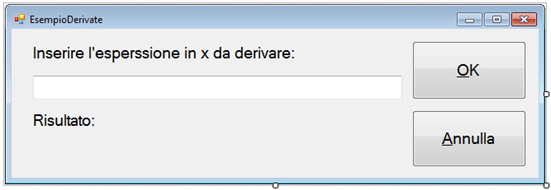
\includegraphics[width=12cm]{images/dotnet-visualstudio3}\\
  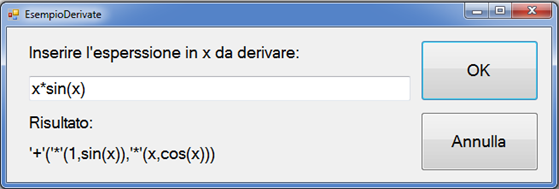
\includegraphics[width=12cm]{images/dotnet-visualstudio5}
  \caption{Creating a .NET application using \tuprolog{} in Visual Studio: the user GUI}\label{fig:dotnet-visualstudio3}
\end{figure}

\begin{figure}
\centering
  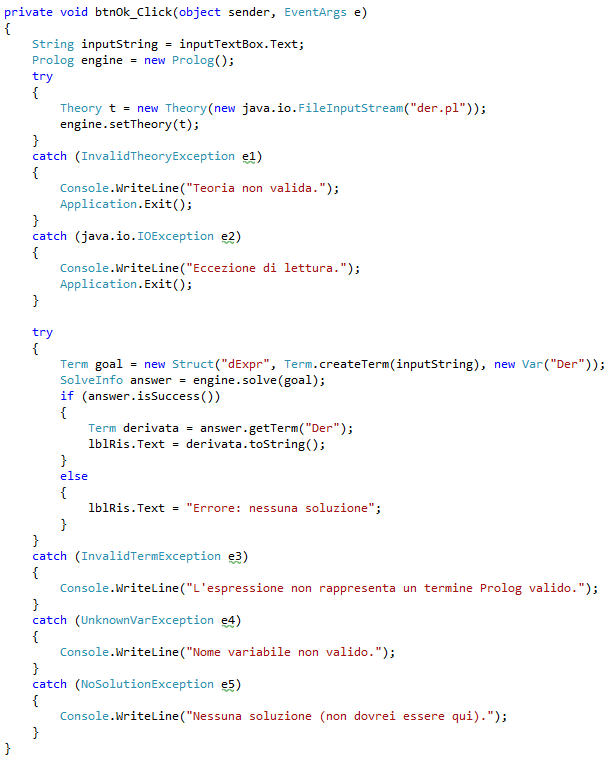
\includegraphics[width=12cm]{images/dotnet-visualstudio4}
  \caption{Creating a .NET application using \tuprolog{} in Visual Studio: the .NET handler of the \textit{OK} button.}\label{fig:dotnet-visualstudio4}
\end{figure}


%-----------------------------------------------------------------------
\section{Augmenting Prolog via .NET:\\developing new libraries}
\label{sec:dotnet-developing new libraries}
%-----------------------------------------------------------------------

New \tuprolog{}.NET libraries can be written in any of the .NET languages, and then compiled normally via Microsoft Visual Studio; alternatively, libraries written in Java can be used, by translating them in .NET via IKVM (if they are not part of the standard \tuprolog{} distribution, of course).

The approach is the basically same presented in Section \ref{sec:howto-develop-libraries} (same method conventions, same need to extend \texttt{alice.tuprolog.Library}), etc.: the only difference concerns how libraries are located in the file system, which obviously adheres to the .NET conventions\footnote{
\texttt{http://msdn.microsoft.com/en-us/library/yx7xezcf.aspx}}.
Accordingly, the configuration file \texttt{2p.exe.config} specifies the custom paths where the library probing must take place: currently, the \texttt{lib} folder is included, so as to provide a standard place where to put any third-party library.
%
If Java classes are also used (\texttt{.class} or \texttt{.jar}), these must be in the same folder as the \texttt{2p.exe} executable (subdirectories are not acceptable).

For instance, if the TestLibrary shown in Section \ref{tab:TestLibrary} on page \pageref{tab:TestLibrary} is translated via IKVM\footnote{Command: \texttt{ikvmc -r:2p.exe TestLibrary.class}} obtaining \texttt{TestLibrary.dll}, the \tuprolog{}.NET GUI can load it directly either via \texttt{load\_library/1}, using its full name \texttt{'TestLibrary, TestLibrary'}, or via the Library Manager dialog, specifying \texttt{TestLibrary, TestLibrary} (without quotes) as the class name (Figure \ref{fig:dotnet-testlibrary}), provided that \texttt{TestLibrary.dll} is in one of the folders where \tuprolog{} is instructed to search---e.g. the \texttt{lib} subfolder.

\begin{figure}
    \centering
  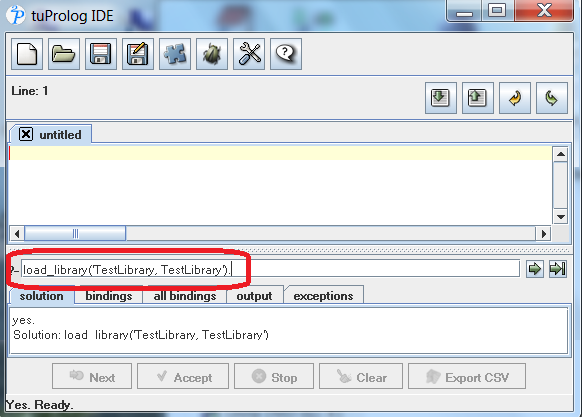
\includegraphics[width=8cm]{images/dotnet-testlibrary1}
  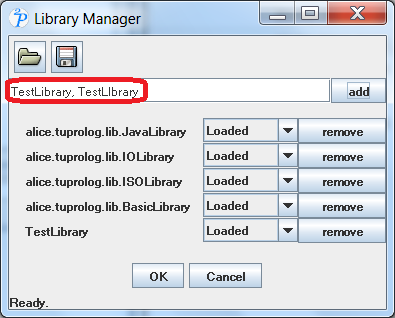
\includegraphics[width=8cm]{images/dotnet-testlibrary2}
  \caption{Loading the translated TestLibrary in the \tuprolog{}.NET GUI either via the \texttt{load\_library} predicate \textit{(top)} or via the library manager \textit{(bottom)}. (Compare with Figures \ref{fig:testlibrary3} and \ref{fig:testlibrary5} on page \pageref{fig:testlibrary5}.)}\label{fig:dotnet-testlibrary}
\end{figure}

\subsection{Capturing exceptions raised in .NET libraries}

Unlike the .NET (and Java's) OOLibrary, where the exceptions possibly raised during a call to some method call can be perceived and caught via the \texttt{java\_catch/3} (or any future renamed version) predicate (Section \ref{ssec:dotnet-oolibrary-exceptions}), the exceptions possibly raised inside a library (in this case, written in .NET) cannot be caught at all, since they have nothing to do with the OOLIbrary filter.
So, if any such exception occurs inside a library, the corresponding predicate simply fails.

\subsection{Capturing the .NET output in Prolog}

Like the Java case, the output possibly performed by the user library is \textit{not} captured in the \tuprolog{}.NET GUI (the engine simply replies \texttt{yes}), because a .NET windows application is not connected to any terminal: even when launched by a command prompt, the app releases the terminal immediately, so no standard output is defined.
This means that, unlike the Java case, any output possibly performed from .NET predicates does not go to the terminal even if there is one---it simply gets lost. So, the only way to perform output is via the Prolog \texttt{write/1} predicate.



%-----------------------------------------------------------------------
\section{Augmenting .NET via Prolog:\\the P@J framework revised}
\label{sec:dotnet-pj}
%-----------------------------------------------------------------------

Since \tuprolog{}.NET is automatically generated from the Java sources via IKVM, the P@J framework presented in Section \ref{sec:p@j} is also available.
%
However, due to intrinsic differences between Java types and .NET types (with special regard to the different handling of generic types in the two platforms), the operativity of the translated P@J in .NET is only partial: to fully exploit the P@.NET functionalities in the .NET world, a new approach has been set up that takes full advantage of advanced features (such as automatic code generation) supported by Microsoft Visual Studio, adopting a different development and computational model while achieving the same conceptual results.

More precisely, the translated P@J in .NET is subject to the following limitations:

\begin{itemize}
  \item a Java application using P@J, translated to .NET via IKVM, works normally in .NET (provided that the proper reference to the translated version of the Javassist library, \texttt{Javassist.dll}, is added to the \texttt{ikvmc} command, as follows:\\
      \texttt{\mbox{~~~}ikvmc -r:2p.exe \textbf{-r:javassist.dll} \textit{App}.class }\\
      whose result, \texttt{App.exe}, is ready to be executed;

  \item instead, a .NET application trying to use P@J via .NET attributes (the .NET counterpart of Java annotations) fails, resulting into an exception in the Javassist tool, because of the incompatible handling of generic types in Java and .NET.
\end{itemize}

\noindent The reason of the above malfunctioning is rooted in the \textit{type erasure} technique adopted by the Java compiler to support generic types without changing the underlying Java Virtual Machine (JVM): with this approach, generic type information is only exploited by the compiler for type checking, but is removed in the generated bytecode, where generic types are replaced with \texttt{Object} or more constrained types (e.g. \texttt{Comparable}, \texttt{Serializable}, etc) when appropriate. While this guarantees that the new code can run on unmodified an JVM, it also implies that generic type information is no longer available at run time.
This is typically unperceived when programming on the Java side alone (except in some particular situations that cannot be discussed here), but does become relevant when interacting with other environments and languages that adopt a different strategy: this is precisely the case of .NET, whose intermediate language does maintain generic type information at run time, too.
As a result, Java methods exploiting generic types will not match analogous .NET methods (e.g, C\# methods) at run time, because the Java compiler erases such type information changing the method signatures: consequently, the translated .NET methods produced by IKVM will also adopt the modified signature -- as there is nothing that IKVM can do reconstruct the removed type information.
In our context, this turns out in the translated P@J being unable to interact with the ``expected'' .NET methods, since, in any sense, such methods are have different signatures.

Quite clearly, the nature of the problem makes a patch impossible, since type inference and generics are essential ingredients of the P@J's architecture and computational model. Newer versions of IKVM could not help, either, because the problem is intrinsic to basic language choices.

For this reason, a radically different, .NET specific approach has been developed, which addresses the P@J goal by a totally different perspective.

%-------------------------------------
\subsection{P@.NET via code generators}
\label{ssec:dotnet-code-generators}
%-------------------------------------

The novel approach described in this section, introduced in \tuprolog{} 2.7, is based on the \textit{code generation} feature provided by Microsoft Visual Studio: in particular, the new tool will be provided as a Visual Studio \textit{extension}, easy to deploy and install by double-clicking\footnote{Microsoft Visual Studio (2005+, 2010 suggested) must already be installed.} a self-contained \texttt{.vsix} archive.

Basically, the idea is to replace the run-time approach of P@J -- where the Prolog code inlined in the Java source is captured and executed at run time via Javassist -- with a development-time approach, where the Prolog code is written in a stand-alone (\texttt{.pl}) file, and a suitable .NET class is automatically generated from such code, compiled to a DLL and linked in the project transparently.
%
As a result, the multi-paradigm .NET programmer can develop his/her Visual Studio solution mixing C\# (or VB.NET, etc) and Prolog code, with the Prolog code being \textit{automatically} ``converted to a DLL'' any time the Prolog source file is saved.
In addition, Prolog errors are reported back to Visual Studio, that shows them seamlessly as compilation errors.

The code generator works on standard \tuprolog{} sources -- that is, no modifications are required to make Prolog sources compatible with the tool; moreover, the generated C\# (or VB.NET, etc) class can be customized in its name and namespace. Even more important, the code generator can operate in two modes -- namely, \textit{static} and \textit{dynamic} modes.
In static mode, the Prolog code is encapsulated in the .NET source when the C\# (or VB.NET, etc) class is generated, similarly to P@J's (where the Prolog code is inlined with the Java code); in dynamic mode, instead, the generated C\# (or VB.NET, etc) class contains only the code to load the Prolog source, deferring the actual loading at run time. This makes it possible to dynamically change the Prolog code without affecting the imperative part of the application, and has no counterpart in the classical P@J behaviour.

By default, the generated class adopts the static mode, belongs to the same namespace as the .NET project that contains the Prolog source file, and has the same name as the Prolog source file: so, for instance, a Prolog source file named \texttt{Perm.pl} will lead to a class named \texttt{Perm.cs} belonging to a namespace named after the project name (e.g. \texttt{PrologTestSolution} in Figure \ref{fig:dotnet-codegen1and2} (top).
%
\begin{figure}
\centering
  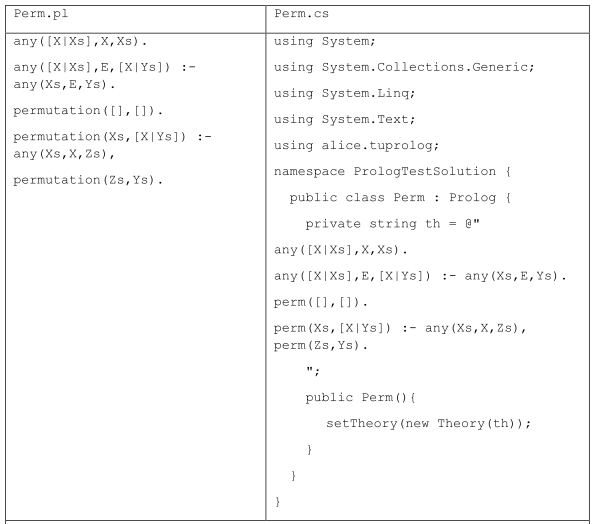
\includegraphics[width=10cm]{images/dotnet-codegen1}\\
  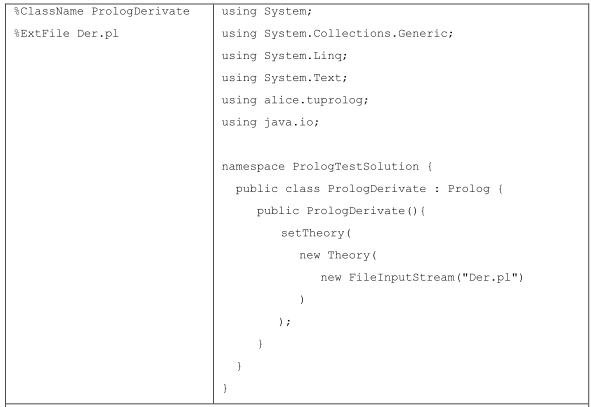
\includegraphics[width=10cm]{images/dotnet-codegen2}
  \caption{Top: generation of a C\# class from the Prolog source (\texttt{Perm.pl}) shown on the left (default, static mode); the new class is named \texttt{Perm.cs}.
  Bottom: same example in the dynamic mode. The Prolog file on the left is now just a pure placeholder containing a reference to the actual Prolog source. The generated class now loads the specified external file instead of embedding the Prolog code as a string.
  }\label{fig:dotnet-codegen1and2}
\end{figure}
%
However, the class generation can be customized by specifying the namespace and/or the class name to be used, annotating the Prolog code with the following meta-information in the form of Prolog comments:

\texttt{\%NameSpace \textit{namespace}}

\texttt{\%ClassName \textit{classname}}

\medskip

\noindent To select the dynamic mode instead of the default static mode:
\begin{itemize}
  \item a placeholder (fake) Prolog file must be included in the Visual Studio project
        instead of the actual Prolog source file;
  \item the placeholder file must contain the meta-information\\
        \mbox{~~~~~~}\texttt{\%ExtFile \textit{prologsource.pl}}\\
        that specifies the name of the actual Prolog source file to be loaded.
\end{itemize}

\noindent Figure \ref{fig:dotnet-codegen1and2} (bottom) shows the example above handled with the dynamic mode: the Prolog file on the left is now the placeholder, containing only the required meta-information for the Prolog generator.

Currently, class templates are provided for C\# and VB.NET only; however, other .NET languages might be supported easily, writing analogous templates and extending \texttt{\textit{PrologGenerator}} to handle the new project type.

%Figure \ref{fig:dotnet-codegen3} shows the flow chart of PrologGenerator, while Figure \ref{fig:dotnet-codegen4} reports the current C\# templates for the static and dynamic modes, respectively.

%\begin{figure}\center
%  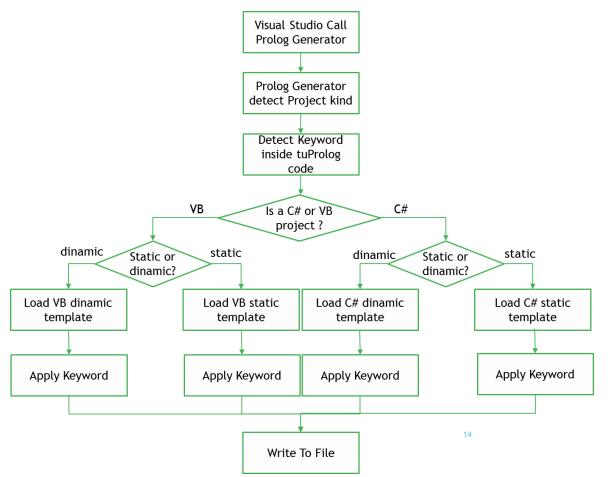
\includegraphics[width=10cm]{images/dotnet-codegen3}
%  \caption{Prolog Generator flow chart.}\label{fig:dotnet-codegen3}
%\end{figure}
%
%\begin{figure}
%  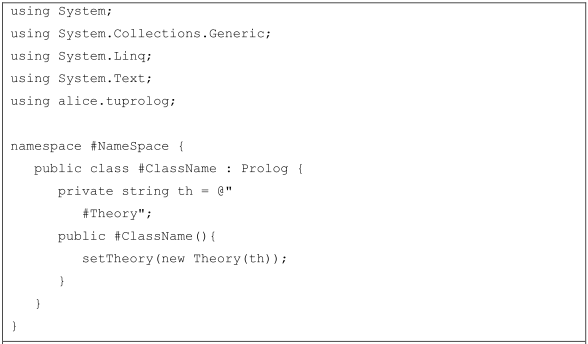
\includegraphics[width=12cm]{images/dotnet-codegen4static}\\
%  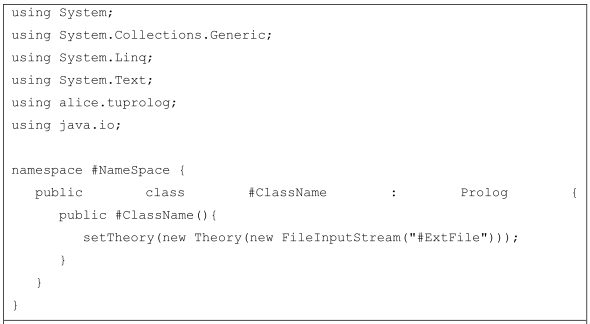
\includegraphics[width=12cm]{images/dotnet-codegen4dynamic}
%  \caption{C\# templates for class generation: static mode (top) and dynamic mode (bottom).}\label{fig:dotnet-codegen4}
%\end{figure}

%-----------------------------------------------------------------------
\section{Putting everything together}
\label{sec:dotnet-putting-together}
%-----------------------------------------------------------------------

As anticipated in Section \ref{sec:dotnet-oolibrary-examples}, interoperability between .NET and Java classes occurs transparently via \tuprolog{}.NET only as long as primitive data types are involved; a problem occurs, instead, when complex types (like lists, arrays, etc.) are asked to cooperate in the same \tuprolog{} program, because a Java object, possibly returned from a Java method, cannot be passed to a .NET instance ``as is'' (and vice-versa), and no automatic conversion occurs.
The typical workaround to this problem is to transform the problematic data in suitable Prolog strings that constitute a valid \tuprolog{} representation of a value of a Prolog type (and viceversa), exploiting \tuprolog{} as a mediator (both as a component and as a language) to overcome the incommunicability.

Suppose, for instance, that two libraries -- one written in Java, the other in some .NET language -- are to be used together in some application.
To exploit \tuprolog{}.NET as a mediator, the critical data to be exchanged must be first serialized into suitable Prolog strings, and then converted into Prolog terms that become the \textit{lingua franca} for data exchange.
The reason for choosing a string based representation is that, beyond its easy applicability to virtually any data type, it can exploit the \texttt{text\_term/2} predicate (which transforms a Prolog term into its textual representation according to pre-defined rules, and viceversa) for speeding up the job and/or perform other intermediate transformations.

These adapter functions can be either encapsulated in the libraries, if their source is available and can be modified, or be put in some \textit{ad hoc} converter classes (Java / .NET depending on the situation), or even be performed directly in Prolog, if the conversion can be more conveniently done in this way.

\begin{figure}
   \centering
  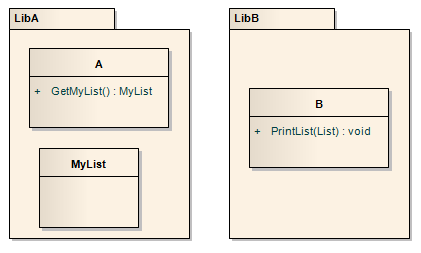
\includegraphics[width=7cm]{images/dotnet-pipolo1}
  \caption{Using \tuprolog{}.NET to bridge between classes using heterogeneous data types.}\label{fig:dotnet-pipolo1}
\end{figure}

Figure \ref{fig:dotnet-pipolo1} shows this kind of situation: class \texttt{A} exposes the \texttt{GetMyList} method that return an instance of \texttt{MyList}, while class \texttt{B} provides a \texttt{PrintList} method that accepts a \texttt{List} instance (not a \texttt{MyList}, then).
Using \tuprolog{} as a mediator/adapter means \textit{a)} to develop the required pair of serialize/deserialize methods, and \textit{b)} exploit \tuprolog{} to bridge class A and B via such methods.
In this case, \texttt{MyListToString} and \texttt{StringToList} are needed to convert \texttt{MyList} to string, and string to \texttt{List}, respectively.
%
If both classes \texttt{A} and \texttt{B} are .NET classes, the best option is probably to implement them as static operations of a third \texttt{Converter} .NET class; if, instead, the two classes belong to different platforms, two different converter classes need to be set up---one in Java, to host \texttt{MyListToString}, and one in .NET, to host \texttt{StringToList}.

The resulting Prolog code would them be something like this:
\begin{verbatim}
    ...
    A <- GetMyList returns MyList,
    Converter1 <- MyListToString(MyList) returns MyListAsText,
    % any intermediate transformation
    Converter2 <- StringToList(ListAsText) returns List,
    B <- PrintList(List),
    ...
\end{verbatim}


%----------------------------------------------
\subsection{Example: Multi-language TicTacToe}
\label{ssec:mpp-tictactoe}
%----------------------------------------------

This example aims to show the data exchange issue between .NET and Prolog in the context of a multi-paradigm application. To this end, the different aspects are assigned to different languages, as follows:
\begin{itemize}
  \item C\# is used for the main entry point (\texttt{tictactoe.exe} file, Figure \ref{fig:dotnet-pipolo5});
  \item a .NET language is used for the data model and I/O handling, i.e. the \texttt{TicTacToe} class: this class is actually implemented in different versions using different languages (C\#, VB.NET, F\# and Java), to test interoperability in different situations (Figure \ref{fig:dotnet-pipolo2});
  \item Prolog is used to express the game logic, i.e. the move generation: this part is coded in the \texttt{tictac.pl} file (Figure \ref{fig:dotnet-pipolo34}).
\end{itemize}

\begin{figure}[h]
   \centering
  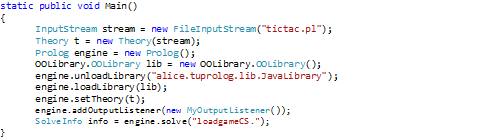
\includegraphics[width=14cm]{images/dotnet-pipolo5}
  \caption{The \texttt{Main} class in C\#: in this case, the C\# version of the \texttt{TicTacToe} class is loaded (last line), but this argument could easily be taken from the command line. Note the loading of \texttt{OOLibrary} and the capturing of Prolog code with the same technique presented in Section \ref{ssec:capturing-output}.}
  \label{fig:dotnet-pipolo5}
\end{figure}

\begin{figure}
   \centering
  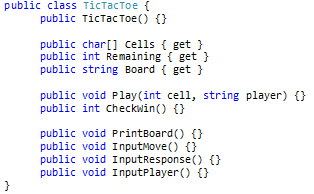
\includegraphics[width=9cm]{images/dotnet-pipolo2}
  \caption{The \texttt{TicTacToe} class: public interface.}\label{fig:dotnet-pipolo2}
\end{figure}

\begin{figure}
   \centering
  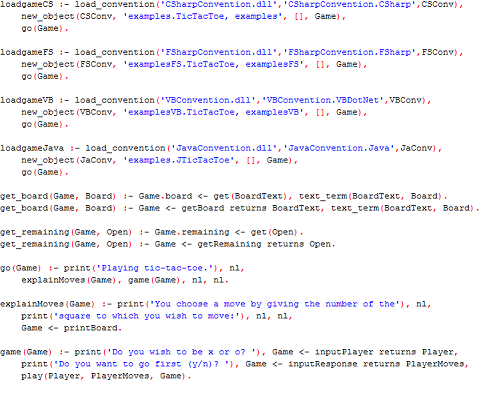
\includegraphics[width=13cm]{images/dotnet-pipolo3}
  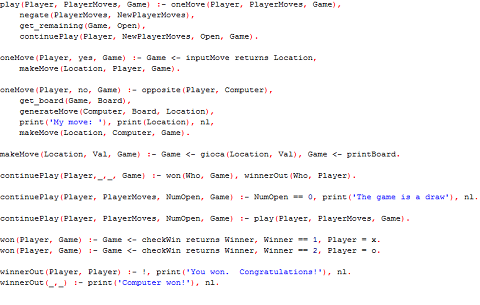
\includegraphics[width=13cm]{images/dotnet-pipolo4}
  \caption{The Prolog code implementing the application logic.}\label{fig:dotnet-pipolo34}
\end{figure}

\noindent In particular, the \texttt{Cells} property returns an array of \texttt{char} that represents the status of the game, each cell being  \texttt{'x'}, \texttt{'o'} or a number in the range 1--9 (the cell number) if it is still free, while the \texttt{Board} property returns the above status in the form of a string interpretable as a Prolog term---namely, something like \texttt{'board(\_,x,o,x,\_,\_,\_,o,x)'}.
In turn, this format is used by the Prolog logic to generate the computer moves.

The \texttt{Play} method receives the cell number and the player (one of \texttt{'x'}, \texttt{'o'} as a string), while \texttt{CheckWin} checks whether some has won (0 meaning no one, 1 meaning that the winner is player \texttt{'x'}, 2 that it is player \texttt{'o'}).
The other methods are self-explaining.

In the Java version, the above properties are replaced by suitable methods; this difference is handled by embedding in the Prolog logic two versions of the \texttt{get\_board} and \texttt{get\_remaining} predicates, that differ only for this aspect: in particular, the first predicate converts the input string into a \texttt{board/9} term via the \texttt{text\_term} library predicate.

The application is launched by one of the \texttt{loadgameCS}, \texttt{loadgameVB}, \texttt{loadgameFS}, \texttt{loadgameJava} methods, that are identical except for loading the \texttt{TicTacToe} class of the corresponding language.
%
Then, the app prompts the user for the preferred placeholder (the preference is stored in the \texttt{Player} variable) and asks whether he/she likes to move first, or not: \texttt{PlayerMoves} contains yes/no depending whether it is the human player's turn to play.
%
The actual move logic is embedded in \texttt{oneMove}, which has two alternative implementations---one for the computer, and one for the human player: both use \texttt{get\_board} above to get the game status. The computer move is generated by \texttt{generateMove}.

Interestingly, the Prolog output is captured with the same approach presented in Section \ref{ssec:capturing-output}, defining the \texttt{MyOutputListener} class as follows:

\begin{verbatim}
   public class MyOutputListener : OutputListener {
     public void onOutput(OutputEvent e) {
        System.Console.Write(e.getMsg());
     }
   }
\end{verbatim}

\noindent The data exchange issue is evident here in the case of the game status: the array is serialized to a string and converted into the desired Prolog term. The opposite conversion (Prolog back to .NET or Java) is not necessary in this application.
The other arguments are of primitive types, so no conversions are needed.
